% This file is part of GUFI, which is part of MarFS, which is released
% under the BSD license.
%
%
% Copyright (c) 2017, Los Alamos National Security (LANS), LLC
% All rights reserved.
%
% Redistribution and use in source and binary forms, with or without modification,
% are permitted provided that the following conditions are met:
%
% 1. Redistributions of source code must retain the above copyright notice, this
% list of conditions and the following disclaimer.
%
% 2. Redistributions in binary form must reproduce the above copyright notice,
% this list of conditions and the following disclaimer in the documentation and/or
% other materials provided with the distribution.
%
% 3. Neither the name of the copyright holder nor the names of its contributors
% may be used to endorse or promote products derived from this software without
% specific prior written permission.
%
% THIS SOFTWARE IS PROVIDED BY THE COPYRIGHT HOLDERS AND CONTRIBUTORS "AS IS" AND
% ANY EXPRESS OR IMPLIED WARRANTIES, INCLUDING, BUT NOT LIMITED TO, THE IMPLIED
% WARRANTIES OF MERCHANTABILITY AND FITNESS FOR A PARTICULAR PURPOSE ARE DISCLAIMED.
% IN NO EVENT SHALL THE COPYRIGHT HOLDER OR CONTRIBUTORS BE LIABLE FOR ANY DIRECT,
% INDIRECT, INCIDENTAL, SPECIAL, EXEMPLARY, OR CONSEQUENTIAL DAMAGES (INCLUDING,
% BUT NOT LIMITED TO, PROCUREMENT OF SUBSTITUTE GOODS OR SERVICES; LOSS OF USE,
% DATA, OR PROFITS; OR BUSINESS INTERRUPTION) HOWEVER CAUSED AND ON ANY THEORY OF
% LIABILITY, WHETHER IN CONTRACT, STRICT LIABILITY, OR TORT (INCLUDING NEGLIGENCE
% OR OTHERWISE) ARISING IN ANY WAY OUT OF THE USE OF THIS SOFTWARE, EVEN IF
% ADVISED OF THE POSSIBILITY OF SUCH DAMAGE.
%
%
% From Los Alamos National Security, LLC:
% LA-CC-15-039
%
% Copyright (c) 2017, Los Alamos National Security, LLC All rights reserved.
% Copyright 2017. Los Alamos National Security, LLC. This software was produced
% under U.S. Government contract DE-AC52-06NA25396 for Los Alamos National
% Laboratory (LANL), which is operated by Los Alamos National Security, LLC for
% the U.S. Department of Energy. The U.S. Government has rights to use,
% reproduce, and distribute this software.  NEITHER THE GOVERNMENT NOR LOS
% ALAMOS NATIONAL SECURITY, LLC MAKES ANY WARRANTY, EXPRESS OR IMPLIED, OR
% ASSUMES ANY LIABILITY FOR THE USE OF THIS SOFTWARE.  If software is
% modified to produce derivative works, such modified software should be
% clearly marked, so as not to confuse it with the version available from
% LANL.
%
% THIS SOFTWARE IS PROVIDED BY LOS ALAMOS NATIONAL SECURITY, LLC AND CONTRIBUTORS
% "AS IS" AND ANY EXPRESS OR IMPLIED WARRANTIES, INCLUDING, BUT NOT LIMITED TO,
% THE IMPLIED WARRANTIES OF MERCHANTABILITY AND FITNESS FOR A PARTICULAR PURPOSE
% ARE DISCLAIMED. IN NO EVENT SHALL LOS ALAMOS NATIONAL SECURITY, LLC OR
% CONTRIBUTORS BE LIABLE FOR ANY DIRECT, INDIRECT, INCIDENTAL, SPECIAL,
% EXEMPLARY, OR CONSEQUENTIAL DAMAGES (INCLUDING, BUT NOT LIMITED TO, PROCUREMENT
% OF SUBSTITUTE GOODS OR SERVICES; LOSS OF USE, DATA, OR PROFITS; OR BUSINESS
% INTERRUPTION) HOWEVER CAUSED AND ON ANY THEORY OF LIABILITY, WHETHER IN
% CONTRACT, STRICT LIABILITY, OR TORT (INCLUDING NEGLIGENCE OR OTHERWISE) ARISING
% IN ANY WAY OUT OF THE USE OF THIS SOFTWARE, EVEN IF ADVISED OF THE POSSIBILITY
% OF SUCH DAMAGE.



\section{Rollup}
\label{sec:rollup}
After an index is created, the index may be rolled up. Rolling up is a
major optimization that can reduce the number of directories that need
to be opened when querying by significant amounts while still
obtaining the same results as an unmodified index.

\subsection{Bottlenecks}
During querying, every single directory runs a fixed set of
operations:

\begin{itemize}
  \item \texttt{opendir(3)}
  \item \texttt{readdir(3)} (Looped)
  \item \texttt{sqlite3\_open\_v2}
  \item \texttt{sqlite3\_exec\_v2}
  \item \texttt{sqlite3\_close(3)}
  \item \texttt{closedir(3)}
\end{itemize}

Each of these operations have costs associated with them. Some are
fixed and some depend on the shape and contents of the index. Reducing
the number of directories processed allows for fixed costs to be
amortized.

\subsection{Rules}
\label{rolluprules}
\subsubsection{Whether or not a directory {\it CAN} roll up}
In order for a child directory to be allowed to roll up into its
parent directory, it must follow two rules. First, all of its children
must be rolled up. Second, all of its children must have permissions
that satisfy any one of the following conditions with the parent.

\begin{itemize}
  \item World readable and executable (o+rx)
  \item Matching user, group, and others permissions, with the same
    user and group
  \item Matching user and group permissions, readable and executable
    (ug+rx) with the same user and group, and not world readable and
    excutable (o-rx)
  \item Matching user permissions, readable and executable (u+rx) with
    the same user and not group or world readable and executable
    (go-rx)
\end{itemize}

Note that because leaf directories have no children with which to have
conflicting permission with, they are considered rolled up.

\subsubsection{Whether or not a directory {\it SHOULD} roll up}
In addition to the permission-based rules that determine whether or
not a directory can roll up, we also have a small check to say whether
or not a directory should roll up.

As data is rolled upwards in the index, databases towards the top will
accumulate more and more data from its subtrees. If directories are
allowed to roll up without limit, some databases will become
significantly larger than others, causing large amounts of tail
latency.

The \rollup executable has the \texttt{-L} flag that limits the number
of entries that may be found within a single directory.

\subsection{Steps}
The processing of rolling up involves a number of steps that update
the tables of the parent directory.

First, the target directory is checked to ensure it can and should
roll up its children into itself using the rules listed in
\ref{rolluprules}. If rollup will proceed, the parent's \summary table
is updated with a rollup score of 1.

Then, the contents each child is copied into the parent:

\begin{enumerate}
\item The child's \pentries view is copied into the parent's
  \pentriesrollup table. The parent's \pentries view is updated
  automatically.
\item The child's \summary table is copied into the parent's \summary
  table with the names of each child directory prefixed with the parent's
  name.
\end{enumerate}

Rolling up can be viewed as flattening the contents of the index while
taking into consideration the permissions of each directory.

Rolling up will cause the size of the index to grow significantly due
to the amount of data being replicated. One obvious optimization would
be to only roll up to the top-most level where a directory can roll up
to (one extra copy of the subtree instead of repeated copies). This
however, will only allow for queries to take advantage of rollups if
they start above the top-most rollup directory. Starting a query below
the top-most rollup level would result in the original subtree's query
time whereas the implemented method of rolling up allows for queries
starting at any point in the index to take advantage of rollups.

The rollup operation can take some time, and so indicies are not
rolled up automatically. The \rollup executable must be called
manually.

\begin{figure} [!h]
  \centering
  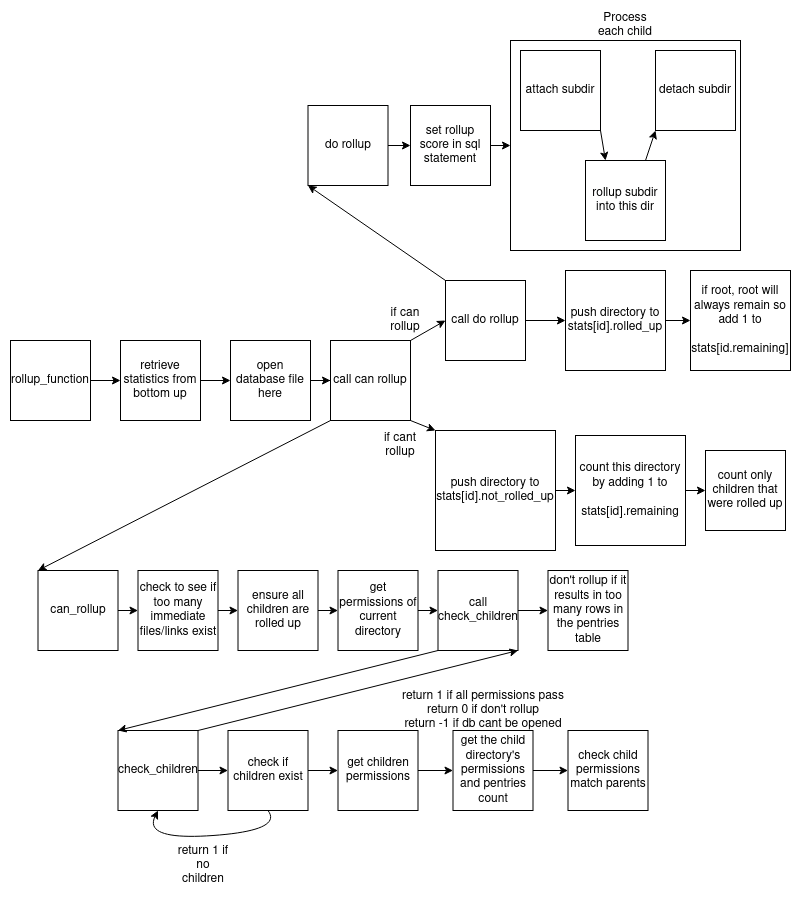
\includegraphics[width=\textwidth]{images/rollup_function.png}
  \caption{Rollup Function Diagram}
\end{figure}

\subsection{\rollup executable}
In order to apply rollup to an index, run the \rollup executable:
\\\\
\indent \rollup \texttt{[index root]}
\\\\
Figure~\ref{fig:rollupworkflow} shows the overall structure of the \rollup
executable. The \rollup executable uses the BottomUp code (see
Section~\ref{sec:bottomup}) to recursively descend the original index and only
perform the rollup operation once all children have been processed.

\begin{sidewaysfigure} [!h]
  \centering 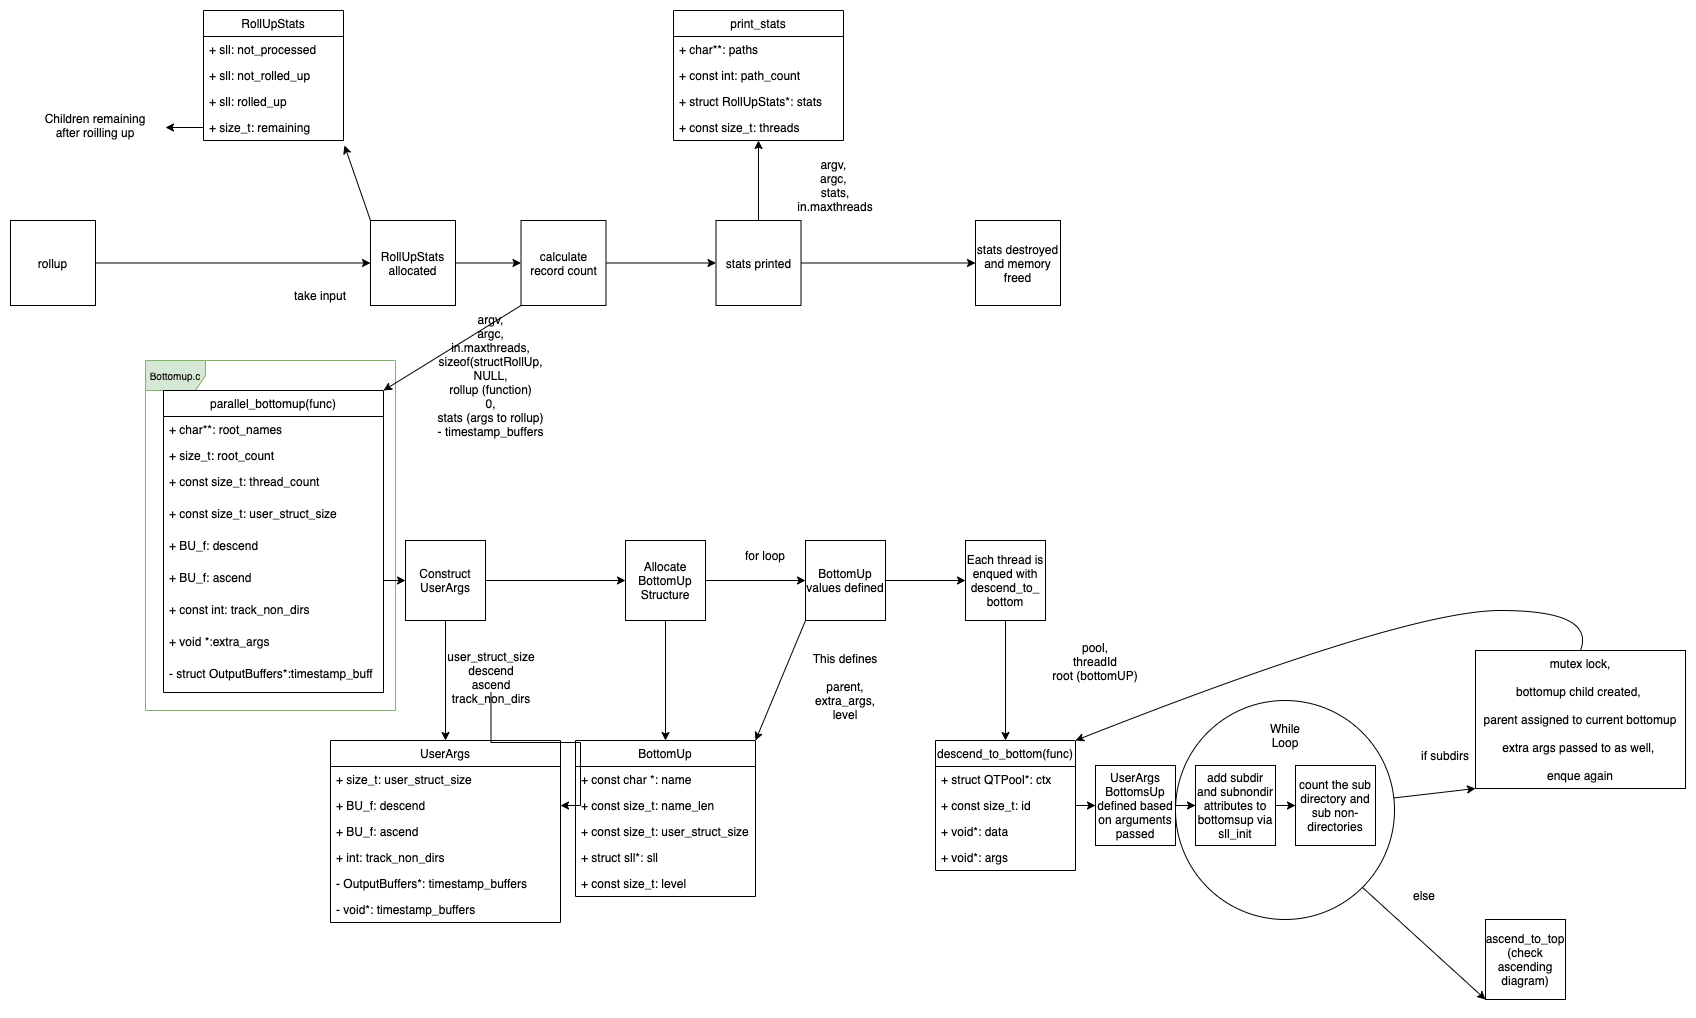
\includegraphics[width=\textwidth]{images/rollup.png}
  \caption{\rollup Workflow}
  \label{fig:rollupworkflow}
\end{sidewaysfigure}

\subsection{Undoing a rollup}
To remove rollup data from an index, run the \unrollup executable:
\\\\
\indent \unrollup \texttt{[index root]}
